\documentclass[a4paper,12pt]{article}
\usepackage{outline}
\usepackage{pmgraph}
\usepackage[normalem]{ulem}
\usepackage{comment} % enables the use of multi-line comments (\ifx \fi)
\usepackage{lipsum} %This package just generates Lorem Ipsum filler text.
\usepackage{fullpage} % changes the margin
\usepackage{listings}
\usepackage{color}
\usepackage{mdframed}
\usepackage{listings}
\usepackage{amssymb}
\usepackage{float}
\usepackage{amsmath}
\usepackage{graphicx}
\usepackage{enumerate,mdwlist}
\graphicspath{ {img/} }
\newenvironment{nscenter}
 {\parskip=0pt\par\nopagebreak\centering}
 {\par\noindent\ignorespacesafterend}

\renewcommand{\lstlistingname}{Code Block}% Listing -> Algorithm
\renewcommand{\lstlistlistingname}{List of \lstlistingname s}% List of Listings -> List of Algorithms

\linespread{1.5}
%--------------------Indention
\setlength{\parindent}{15pt}
\lstset{frame=shadowbox, rulesepcolor=\color{white}}
\mdfsetup{frametitlealignment=\center}
\lstset{
  numbers=left,
  stepnumber=1,
  firstnumber=1,
  numberfirstline=true
}

\begin{document}
\begin{nscenter}
  Project 1 \\
  Joseph Martinsen \\
  Math 308-510 \vspace{35pt}
\end{nscenter}
STATEMENT OF PROBLEM: Consider the following differential equations:

\begin{enumerate}[I.]
  \item $\dfrac{dy}{dx} = xy$
  \item $\dfrac{dy}{dx} = y^2$
  \item $x \dfrac{dy}{dx} + \sin(x)y = x^2$
  \begin{enumerate}[1.]
    \item Graph the direction field in the neighborhood of the origin
    \item Graph approximate integral curves for 10 different initial conditions (you can use dfield8.m)
    \item Solve the differential equation using Euler's method (e.g. with euler.m), for three initial conditions and two values of the stepsize, h
    \item If possible compute the error, either using the exact solution (if available) or a very accurate numerical solution (from Matlab)
  \end{enumerate}
\end{enumerate}

\begin{enumerate}[I.]
  \item Using Matlab, we investigate the following differential equation
  \begin{align*}
    \dfrac{dy}{dx} = xy
  \end{align*}
  \begin{enumerate}[a)]
    \item \textbf{Direction Field.} The direction field near the origin, $-5 \leq x \leq 5. -5 \leq y \leq 5$ is shown below
    \begin{figure}[H]
      \begin{center}
        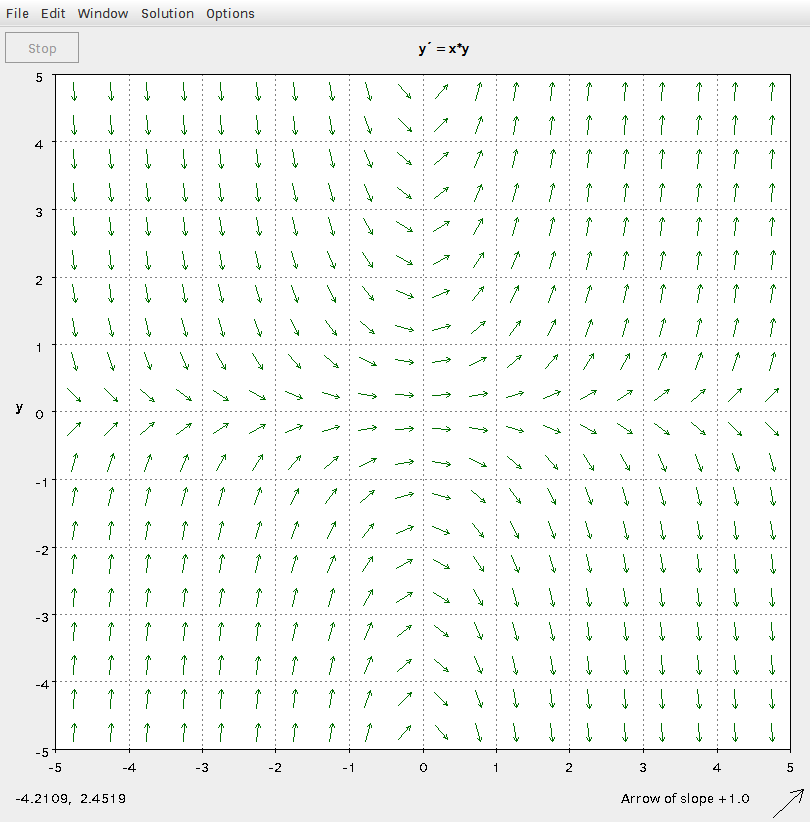
\includegraphics[scale=.3]{11.png}
        \caption{Direction field of $y\;' = xy$}
        \label{fig:1}
      \end{center}
    \end{figure}
    
    \item \textbf{Integral curves.} 10 different initial conditions are shown in the figure below
        \begin{figure}[H]
      \begin{center}
        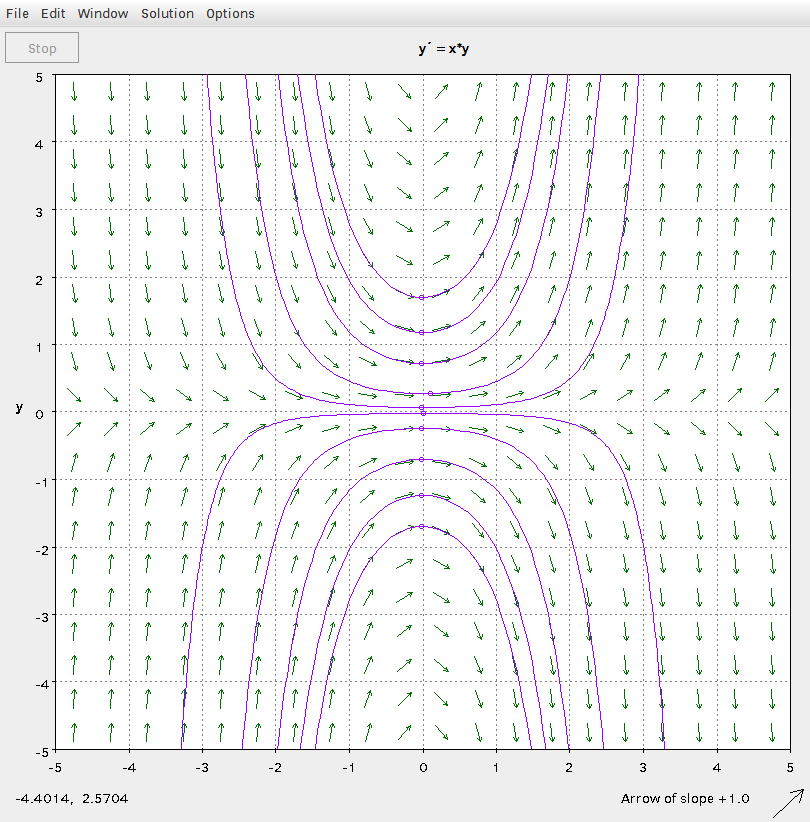
\includegraphics[scale=.3]{12.png}
        \caption{Integral curves of $y\;' = xy$}
        \label{fig:2}
      \end{center}
    \end{figure}
    \item \textbf{Numerical solution.} \\
      The exact solution for $y(0) = 1$ is using Matlab is given by
      \begin{align*}
        \displaystyle y = e^{x^2/2}
      \end{align*}
      
      The graph of the results of Euler's method, with $h=0.1$ and $h=0.01$ is compared to the solution before. \\
      
      \begin{figure}[H]
        \begin{center}
          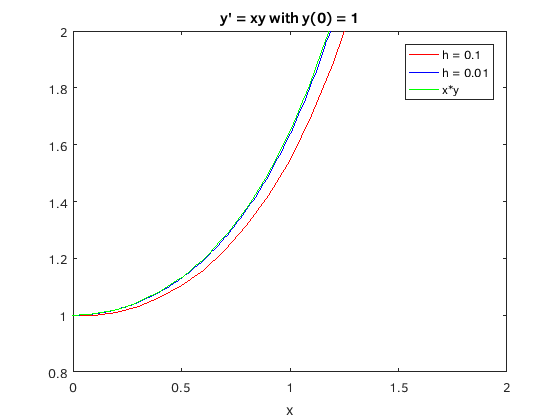
\includegraphics[scale=.9]{111.png}
          \caption{With $y(0)=1$}
        \end{center}
      \end{figure}
      
      The exact solution for $y(0)=2$ found using Matlab is given by
      \begin{align*}
        y = 2e^{x^2/2}
      \end{align*}
      
      The graph of the results of Euler's method, with $h=0.1$ and $h=0.01$, is compared to the exact solution below
      
      \begin{figure}[H]
        \begin{center}
          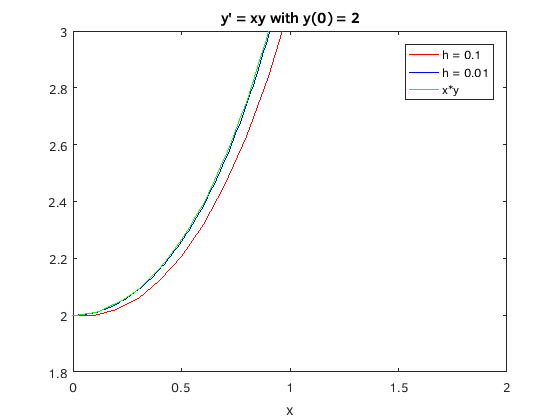
\includegraphics[scale=.9]{112.png}
          \caption{With $y(0) = 2$}
        \end{center}
      \end{figure}
      
      The exact solution for $y(0)=-1$ found using Matlab is given by
      \begin{align*}
        y=-e^{x^2/x}
      \end{align*}

      The graph of the results of Euler's method, with $h=0.1$ and $h=0.01$, is compared to the exact solution below
      
            \begin{figure}[H]
              \begin{center}
                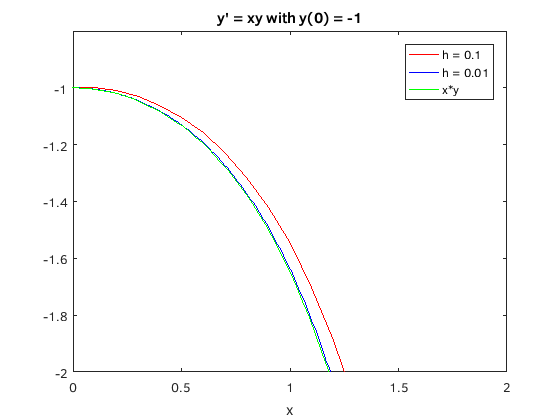
\includegraphics[scale=.9]{113.png}
                \caption{With $y(0) = -1$}
                \label{fig:}
              \end{center}
            \end{figure}
    
    \item  \textbf{Error.} Error, as a function of h. We fix the initial condition, and the interval [0,1], and then compute the error (defined as the maximum of the absolute value of the pointwise error over the interval) versus the step size h. The initial condition being analyzed is for $y(0) = 2$
    
    \begin{table}[H]
      \caption{Error Analysis of $y = 2e^{x^2/2}$}
      \label{tab:}
    
      \begin{center}
        \begin{tabular}{|c|c|}
           \hline
           Step & Max Abs Difference \\
           \hline
           \hline
           .1   & 0.20322 \\
           \hline
           .05  & 0.10556 \\
           \hline
           .01  & 0.00218 \\
           \hline
           .005 & 0.10946 \\
           \hline
           .001 & 0.00220 \\
           \hline
        \end{tabular}
      \end{center}
    \end{table}
    \begin{figure}[H]
      \begin{center}
        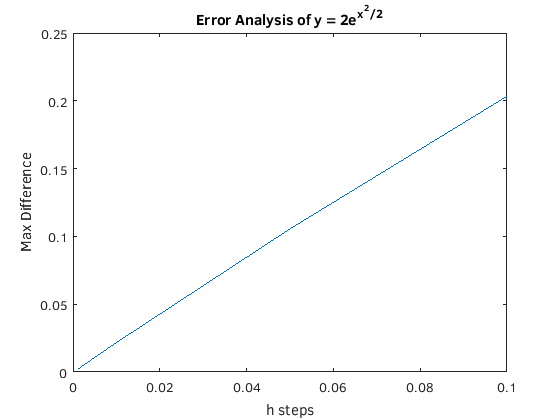
\includegraphics[scale=.9]{114.png}
        \caption{Error Analysis of $y = 2e^{x^2/2}$}
      \end{center}
    \end{figure}
  \end{enumerate}

  \item Using Matlab, we investigate the following differential equation
  \begin{align*}
    \dfrac{dy}{dx} = y^2
  \end{align*}
  \begin{enumerate}[a)]
    \item \textbf{Direction Field.} The direction field near the origin, $-5 \leq x \leq 5. -5 \leq y \leq 5$ is shown below
    \begin{figure}[H]
      \begin{center}
        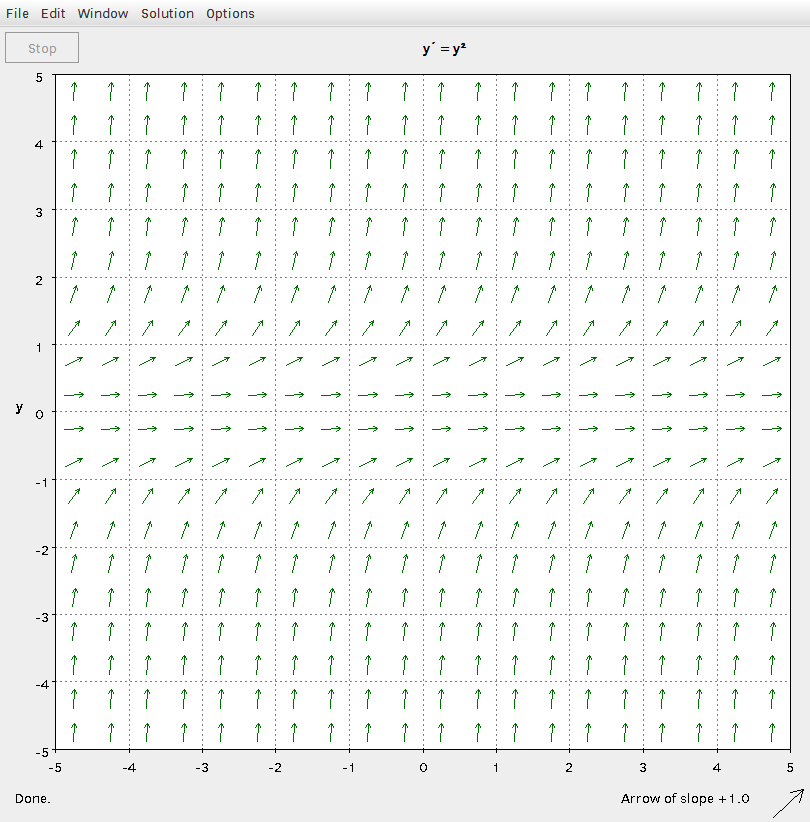
\includegraphics[scale=.3]{21.png}
        \caption{Direction field of $y\;' = y^2$}
        \label{fig:3}
      \end{center}
    \end{figure}
    
    \item \textbf{Integral curves.} 10 different initial conditions are shown in the figure below
        \begin{figure}[H]
      \begin{center}
        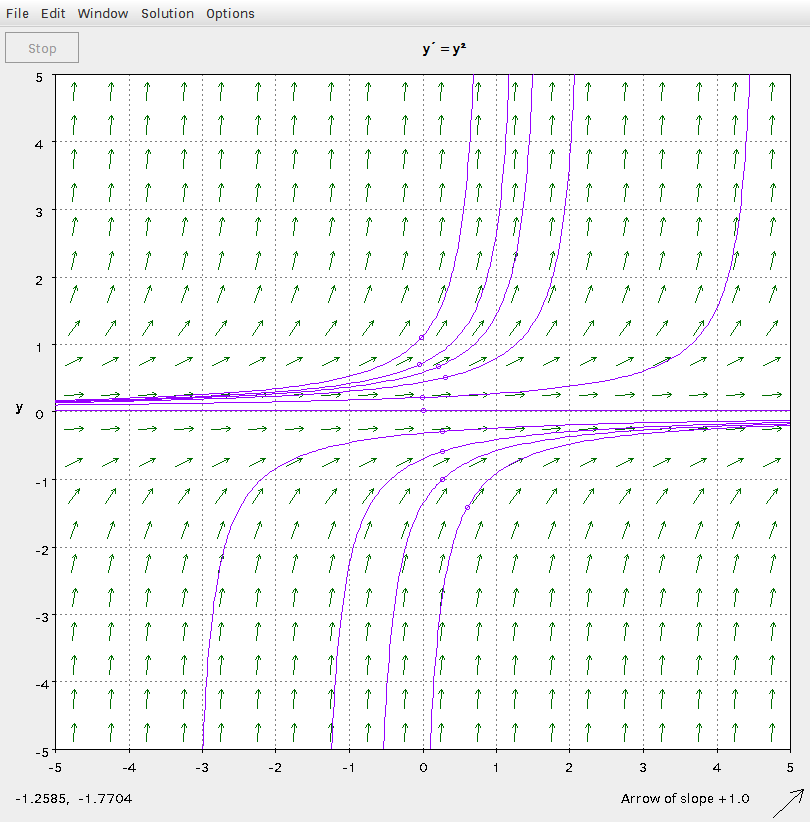
\includegraphics[scale=.3]{22.png}
        \caption{Integral curves of $y\;' = y^2$}
        \label{fig:4}
      \end{center}
    \end{figure}
    \item \textbf{Numerical solution.} \\

      The exact solution for $y(0)=-1$ found using Matlab is given by
      \begin{align*}
        y=- \dfrac{1}{x-1}
      \end{align*}

      The graph of the results of Euler's method, with $h=0.1$ and $h=0.01$, is compared to the exact solution below
      
            %INSERT GRAPH
            
      The exact solution for $y(0)=-1$ found using Matlab is given by
      \begin{align*}
        y=-\dfrac{1}{x - \frac{1}{2}}
      \end{align*}

      The graph of the results of Euler's method, with $h=0.1$ and $h=0.01$, is compared to the exact solution below
      
            %INSERT GRAPH
            
      The exact solution for $y(0)=-1$ found using Matlab is given by
      \begin{align*}
        y=-\dfrac{1}{x+1}
      \end{align*}

      The graph of the results of Euler's method, with $h=0.1$ and $h=0.01$, is compared to the exact solution below
      
            %INSERT GRAPH
            
    \item
  \end{enumerate}
  
  \item Using Matlab, we investigate the following differential equation
  \begin{align*}
    xy\;' + \sin(x)y = x^2
  \end{align*}
  \begin{enumerate}[a)]
    \item \textbf{Direction Field.} The direction field near the origin, $-5 \leq x \leq 5. -5 \leq y \leq 5$ is shown below
    \begin{figure}[H]
      \begin{center}
        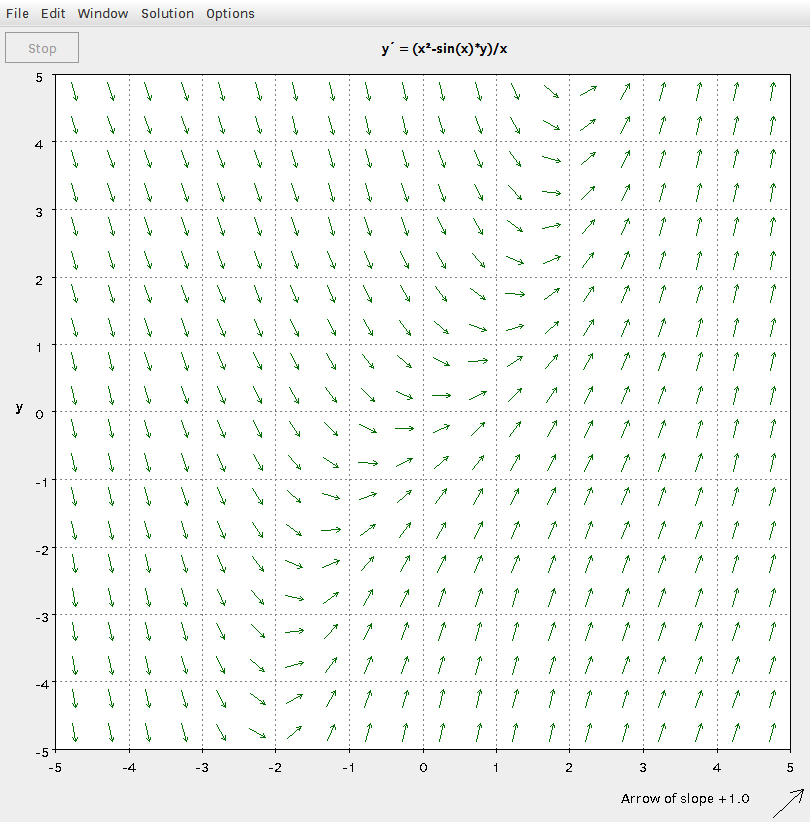
\includegraphics[scale=.3]{31.png}
        \caption{Direction field of $xy\;' + \sin(x)y = x^2$}
        \label{fig:5}
      \end{center}
    \end{figure}
    
    \item \textbf{Integral curves.} 10 different initial conditions are shown in the figure below
        \begin{figure}[H]
      \begin{center}
        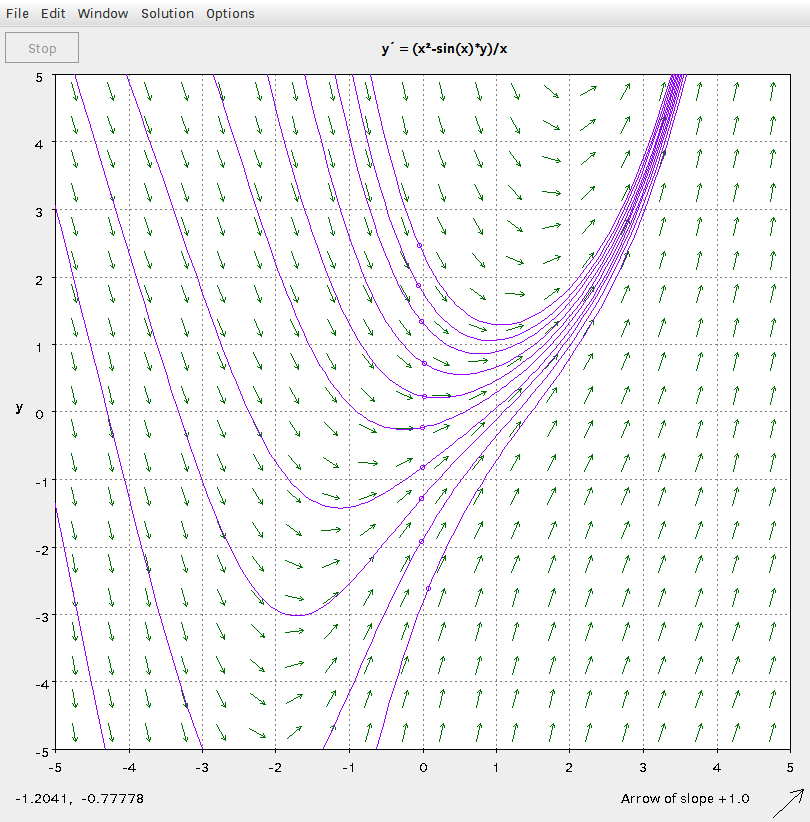
\includegraphics[scale=.3]{32.png}
        \caption{Integral curves of $xy\;' + \sin(x)y = x^2$}
        \label{fig:6}
      \end{center}
    \end{figure}
    \item
    \item
  \end{enumerate}
\end{enumerate}




\end{document}
